% - Privatisation of data
%   - Google, Facebook, NHS, Banks, retail stores (loyalty programs)
%   - Data Protection Act (limitations and corporate-focus)
% - User choice (who do I want to have my data and how)
% - Online identities
%   - Global identity tracking
%   - Conglomerate identity providers
\subsection{Motivation}

At the core of the motivation for this project lay several issues corresponding to the way in which society has been manipulated over time. It is my belief that we find ourselves in the current position without any ownership of our data because we've been keen (even greedy) as a society to reap the benefits of our data without considering the longer term security effects. We have neglected our responsibility to care for our data.

Over the last 350 years, the general public has, often unwittingly, handed their right to privacy over to corporations, conglomerates, and governments through the medium of data transactions. The origin of these transactions in the UK might be attributed to the introduction of paper money in 1694 (\cite{bankofengland:2016:online}). The introduction of paper currency gave an opportunity to the Bank of England to start collecting data on the exchange of money nationally. At the time it is unlikely that any person exchanging gold for paper currency was aware of the impending social shift, likely more concerned with the convenience afforded to them. Before this time, a person might have kept their savings 'under the mattress' and almost certainly would not have shared information relating to their wealth with another party. Whilst bank notes were introduced as a means to raise funds for war, the seed for a data revolution was inadvertently sewn. Whilst no unique identities were shared at this point, they would be in years to come.

Fast forward several hundred years and we find ourselves in a society where it is commonplace to rely on few key corporations and organisations to control information nationally and internationally. As (probably) the world's most popular social network, according to \cite{worldmapsocialnetworks:2017:online}, it is clear from \cite{facebookterms:2015:online} that our use of Facebook's social network is subject to a few key conditions which restrict and change the status quo of our privacy as users. Foremost, it is apparent that whilst content posted on Facebook remains the property of the owner, Facebook has the right to use it how it wishes (as per the IP license) and hence is the controller of that data. One might choose to post their content on Facebook, but one cannot stop Facebook using their content without first removing it from all of Facebook's services and ensuring everyone with whom one has shared the content with has also removed it from Facebook. Furthermore this allows Facebook to use any content posted for machine learning, training systems, and providing commercial services using the intelligence gained from the distribution of content on the Facebook network. As someone who cares for their privacy, it is my opinion that this is not an acceptable status quo.

In addition, Facebook is not the only social network with this perspective on user privacy. \cite{twittertos:2017:online} also shares a very similar stance and it is generally observed with most similar companies.

% TODO: Swiss health identity card data

% - Privatisation of data
%   - Google, Facebook, NHS, Banks, retail stores (loyalty programs)
%   - Data Protection Act (limitations and corporate-focus)
% - User choice (who do I want to have my data and how)
% - Online identities
%   - Global identity tracking
%   - Conglomerate identity providers

To further explain this point, I present three key domains where we, as data owners, lack control. Whilst written as a piece of fiction, we should be aware and concerned that ignoring the social issues with data transfer allows a world to form much similar to that imagined by \cite{orwell:1984:book}.

\subsubsection{Commoditisation of personal (and private) data}

There is no doubt that search tools such as those offered by Google and Microsoft, retail stores such as those offered by Amazon, and social networks such as Facebook and Twitter, dramatically enhance our lives and give us capabilities we would never have otherwise. Often as consumers we are eager to accept these benefits without considering the means by which they are offered to us. Every time we enter a search term into one of the websites above, or we buy something, or even when we click on a particular item in a store, a data point is generated. Whilst not valuable to us as consumers, that data point is the currency of choice of the multinationals. The more data points a corporation has per person, the easier it proves for them to accurately target you with information and offers that you will positively respond to.

For example, \cite{amazoninterestads:2017:online} explains how it uses data gathered from it's own site and any other site where you interact with an Amazon-run entity (such as an advert). Whilst this exchange of data does mean you might receive offers more accustomed to your taste, it somewhat limits consumer choice and is designed such that the corporation makes the maximum profit.

\subsubsection{Retrieval of personal data}

As consumers we are not only exploited through data, but we also receive very little benefit from the data collected about us. Whilst we are able to share content using social networks and distribute this globally, other information is not so easily accessible.

As part of this project, I made a personal request to the NHS to get access to all data kept about myself. At first, the process seemed relatively simple and I hesitate to say that I was suprised. The NHS Digital response to my enquiry suggested that my health records may be available online and indeed this is suggested by the Patient Access service. Upon logging in however, I was greeted with screen in figure \ref{fig:patient_access_services}.

\begin{figure}[H]
  \centering
  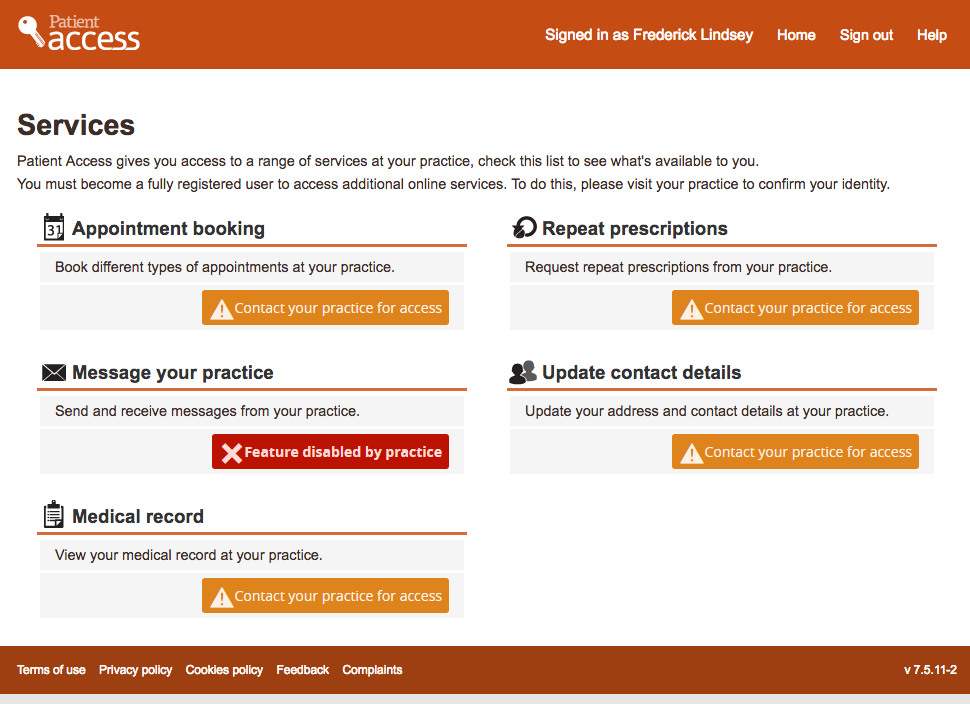
\includegraphics[width = 10cm]{images/patient_access_services.png} \\
  \caption{
  	Patient Access Services
  }{
    The services available to me (as of 13th June 2017) through Patient Access.
  }
  \label{fig:patient_access_services}
\end{figure}


The practice confirmed that whilst they recognise and are connected to the Patient Access service, they have no intention of connecting individual medical records they hold. Whilst it is possible to view your records informally with the supervision and guidance of a doctor, a formal request to receive a copy of the data held on file incurs financial implications\footnote{Data retrieval is at a cost of between £10 and £50 per item depending on its electronic/physical status. \href{https://www.gov.uk/government/publications/subject-access-request}{\textit{HSCIC Subject Request}}}

\subsubsection{Sharing of personal data}

Corporations profit from the aggregation and commoditisation of our data. Furthermore, as expressed, they do not allow the retrieval of our complete data records in an easy and obtainable manner. Therefore, the corporation acting as an intermediatary to share your data also has a vested interest in not allowing you to share your data without them. Fundamentally, there is no way to easily share data without an intermediatary or with an intermdiatary over which you have complete control. Given this, there is never a guarantee that your data is shared privately (i.e. only to parties intended).

Take, for example, an image of a new born baby. It is likely that you would not wish for this image to exist in the public space. Currently, sharing the image requires using a centralised service provided by a corporation who facilitates the sharing process. Through this process you are able to establish, through collusion, whether your data successfully reached the intended recipient. You are not able to confirm that your data was not 'mined' nor viewed by another party, either the corporation itself or a nefarious user. There is no proof of any scheme to encrypt and keep private your data through the transfer process.
